\documentclass{scrartcl}

\usepackage{graphicx}
\usepackage[utf8]{inputenc}
\usepackage[T1]{fontenc}
\usepackage{lmodern}
\usepackage[english]{babel}
\usepackage{amsmath}
\usepackage{amsthm}
\usepackage{mathtools}
\usepackage{amssymb}
\usepackage{listings}
\usepackage{xparse}
\usepackage{geometry}
\usepackage{enumerate}
\usepackage{tikz}
\usepackage{hyperref}
\usepackage[style=english]{csquotes}
\usepackage[language=english, backend=biber, style=alphabetic, sorting=nyt]{biblatex}

\hypersetup{
    colorlinks,
    linkcolor={red!50!black},
    citecolor={blue!50!black},
    urlcolor={blue!80!black}
}

\usetikzlibrary{babel, positioning, shapes.geometric, arrows, arrows.meta}
\addbibresource{bibliography.bib}

\title{Miniproject - Introduction to Schemes}
\author{Simon Pohmann}

\newcommand{\N}{\mathbb{N}}
\newcommand{\Z}{\mathbb{Z}}
\newcommand{\F}{\mathbb{F}}
\newcommand{\C}{\mathbb{C}}
\newcommand{\Q}{\mathbb{Q}}
\newcommand{\I}{\mathbb{I}}
\newcommand{\V}{\mathbb{V}}
\newcommand{\A}{\mathbb{A}}
\renewcommand{\P}{\mathbb{P}}
\newcommand{\p}{\mathfrak{p}}
\newcommand{\q}{\mathfrak{q}}
\newcommand{\m}{\mathfrak{m}}
\renewcommand{\a}{\mathfrak{a}}
\renewcommand{\b}{\mathfrak{b}}
\renewcommand{\m}{\mathfrak{m}}
\newcommand{\Nil}{\mathfrak{N}}
\newcommand{\Set}{\mathrm{\textbf{Set}}}
\newcommand{\Aff}{\mathrm{\textbf{Aff}}}
\newcommand{\Sch}{\mathrm{\textbf{Sch}}}
\newcommand{\Ring}{\mathrm{\textbf{Ring}}}
\newcommand{\Ab}{\mathrm{\textbf{Ab}}}
\newcommand{\Top}{\mathrm{Top}}
\newcommand{\Spec}{\mathrm{Spec}}
\newcommand{\Proj}{\mathrm{Proj}}
\newcommand{\Frac}{\mathrm{Frac}}
\newcommand{\im}{\mathrm{im}}
\newcommand{\cont}{\mathrm{cont}}
\renewcommand{\O}{\mathcal{O}}
\DeclareMathOperator*{\colim}{colim}

\newcommand\restr[2]{{
    \left.\kern-\nulldelimiterspace
    #1
    \vphantom{\big|}
    \right|_{#2}
}}

\newtheorem{prop}{Proposition}
\newtheorem{theorem}[prop]{Theorem}
\newtheorem{lemma}[prop]{Lemma}
\newtheorem{corollary}[prop]{Corollary}

\theoremstyle{definition}
\newtheorem{problem}[prop]{Problem}
\newtheorem{alg}[prop]{Algorithm}
\newtheorem{definition}[prop]{Definition}
\newtheorem{example}[prop]{Example}
\newtheorem{remark}[prop]{Remark}
\newtheorem{reminder}[prop]{Reminder}

\begin{document}
\maketitle

\tableofcontents

\section{Definition of $\Proj$}

\begin{definition}
    A \emph{graded ring} $S$ is a ring $S$ with a decomposition $S = \oplus_{d \in \Z} S_d$ into groups $S_i \subseteq S$ (w.r.t. addition in $S$) such that $S_i S_j \subseteq S_{i + j}$ for all $i, j \in \Z$.
    If all $S_d = \{ 0 \}$ for $d < 0$, call $S$ \emph{naturally graded ring}.
    Write further $S_+ := \sum_{d \neq 0} S_d$.
    For a homogeneous $f \in S_d$ say that $\deg(f) := d$ is its \emph{degree}.

    An element $f \in S$ is called \emph{homogeneous} (of degree $n$), if $f \in S_n$.
    An ideal $I \leq S$ is called \emph{homogeneous}, if it has a set of homogeneous generators.
\end{definition}
\begin{definition}
    For a naturally graded ring $S$, define the set
    \begin{equation*}
        \Proj(S) := \{ \p \in \Spec(S) \ | \ \text{$\p$ homogeneous}, \ S_+ \not\subseteq \p \}
    \end{equation*}
    of homogeneous prime ideals not containing $S_+$.

    This becomes a topological space by endowing it with the \emph{Zariski-topology} on $\Proj(S)$, given by the open sets
    \begin{equation*}
        D_{\a} := \{ \p \in \Proj(S) \ | \ \a \not\subseteq \p \}
    \end{equation*}
    for any homogeneous ideal $\a \leq S$.
\end{definition}
From now on let $S$ be a naturally graded ring.
\begin{prop}
    The above definition is well-defined, i.e. the sets $D_\a$ indeed form a topology on $\Proj(S)$.
\end{prop}
\begin{proof}
    Clearly $\Proj(S) = D_{\langle 1 \rangle}$ and $\emptyset = D_{\langle 0 \rangle}$ are open.
    Furthermore, for open sets $D_\a$ and $D_\b$, have that
    \begin{equation*}
        D_\a \cap D_\b = \{ \p \in \Proj(S) \ | \ \a, \b \not\subseteq \p \} = \{ \p \in \Proj(S) \ | \ \a\b \not\subseteq \p \} = D_{\a\b}
    \end{equation*}
    This holds, as $\a, \b \not\subseteq \p$ implies that there are $f \in \a$ and $g \in \b$ with $f, g \notin \p$.
    However, then $fg \notin \p$ as $\p$ is prime.
    Obviously $\a\b$ is homogeneous, and so $D_\a \cap D_\b$ is open.

    Finally, given a collection $\mathcal{A}$ of homogeneous ideals in $S$, have that
    \begin{align*}
        \bigcup_{\a \in \mathcal{A}} D_\a =& \{ \p \in \Proj(S) \ | \ \exists \a \in \mathcal{A}:\ \a \not\subseteq \p \} = \{ \p \in \Proj(S) \ | \ \exists \a \in \mathcal{A} \exists f \in \a:\ f \notin \p \} \\
        =& \Bigl\{ \p \in \Proj(S) \ \Bigm| \ \exists f \in \sum_{\a \in \mathcal{A}} \a:\ f \notin \p \Bigr\} = D_{\b} \quad \text{for $\b = \sum_{\a \in \mathcal{A}} \a$}
    \end{align*}
    Clearly $\b$ is again homogeneous, and so $\bigcup_{\a \in \mathcal{A}} D_\a$ is open.
\end{proof}
\begin{prop}
    The sets $D_f := D_{\langle f \rangle}$ for homogeneous $f \in S$ form a basis of the topology on $\Proj(S)$.
\end{prop}
\begin{proof}
    Clearly $\langle f \rangle$ is a homogenous ideal, so $D_f$ is open.
    For any homogeneous ideal $\a = \langle f_i \ | \ i \in I \rangle$ with $f_i \in S$ homogeneous have
    \begin{equation*}
        D_\a = \bigcup_{i \in I} D_{f_i}
    \end{equation*}
    as $\a \not\subseteq \p$ implies there is some $g = \sum_{i \in I} g_i f_i \notin \p$, with $g_i \in S$.
    Hence, at least one $g_j f_j \notin \p$ and so $f_j \notin \p$, thus $\p \in D_{f_j}$.
    It follows that the $D_f$ generate the topology on $\Proj(S)$, so it is left to show that they are a basis.

    Consider $\p \in D_f \cap D_g$, so $f, g \notin \p$.
    Since $\p$ is prime, it follows that $fg \notin \p$ and so $D_{fg} \subseteq D_f \cap D_g$ is an open neighborhood of $\p$.
\end{proof}
\begin{lemma}
    Let $S$ be a graded ring (not necessarily naturally graded) and $T \subseteq S$ a multiplicative set consisting of homogeneous elements. 
    Then $T^{-1}S$ becomes a graded ring via
    \begin{equation*}
        \left(T^{-1}S\right)_d = \Bigl\{ \frac g h \in T^{-1}S \ \Bigm| \ \text{$g$ homogeneous with $\deg(g) - \deg(h) = d$} \Bigr\}
    \end{equation*}
\end{lemma}
\begin{proof}
    Clearly $(T^{-1}S)_i (T^{-1}S)_j \subseteq (T^{-1}S)_{i + j}$.
    To see that $(T^{-1}S)_d$ is a subgroup of $S$, consider $g/f, l/h \in (T^{-1}S)_d$.
    Now have
    \begin{equation*}
        \frac g f + \frac l h = \frac {gh + lf} {hf}
    \end{equation*}
    and by assumption, find $\deg(gh) = \deg(g) - \deg(h) = d + \deg(f) - d + \deg(l) = \deg(lf)$.
    So $gh + lf$ is homogeneous and we have
    \begin{equation*}
        \deg(gh + lf) - \deg(fh) = \deg(f) + \deg(l) - \deg(f) - \deg(h) = \deg(l) - \deg(h) = d
    \end{equation*}
    Thus $g/f + l/h \in (T^{-1}S)_d$.

    Finally, we show that $(T^{-1}S)_n \cap (T^{-1}S)_m = \{ 0 \}$ for $i \neq j$.
    Assume there is $g/f = l/h \in (T^{-1}S)_n \cap (T^{-1}S)_m$ with $\deg(g) - \deg(f) = n$ and $\deg(l) - \deg(h) = m$.
    Then there exists $t \in T$ such that
    \begin{align*}
        0 = t(gh - lf) =& tgh - tlf \quad \text{with}\ tgh \in S_{\deg(t) + \deg(g) + \deg(h)} \\
        &\text{and}\ tlf \in S_{\deg(t) + \deg(l) + \deg(f)} = S_{\deg(t) + \deg(g) + \deg(h) + (m - n)}
    \end{align*}
    If $n \neq m$, then $S_{\deg(t) + \deg(g) + \deg(h) + (m - n)} \cap S_{\deg(t) + \deg(g) + \deg(h)} = \{ 0 \}$ and so $tgh = tlf = 0$.
    Thus $th(g - 0) = 0$ and so $g/f = 0/1 = 0$.
    Thus $(T^{-1}S)_m \cap (T^{-1}S)_n = \{ 0 \}$.
\end{proof}
\begin{lemma}
    \label{prop:homogeneous_part_prime}
    Let $\p \leq S$ be a prime ideal.
    Then
    \begin{equation*}
        \p' := \langle f \in \p \ | \ \text{$f$ homogeneous} \rangle \leq S
    \end{equation*}
    is a (homogeneous) prime ideal.
\end{lemma}
\begin{proof}
    Consider $f, g \in S$ with $f g \in \p'$ and assume $f, g \notin \p'$.
    Write $f = \sum_d f_d$ and $g = \sum_d g_d$ with $f_d, g_d \in S_d$.
    So
    \begin{equation*}
        \sum_{i, j} f_i g_j = \sum_n \sum_{i + j = n} f_i g_j \in \p'
    \end{equation*}
    Since $\p'$ is homogeneous, it follows that
    \begin{equation*}
        \sum_{i + j = n} f_i g_j \in \p'
    \end{equation*}
    for all $n \in \Z$.

    Let now $d$ resp. $e$ be maximal such that $f_d \notin \p'$ resp. $g_e \notin \p'$.
    We have
    \begin{equation*}
        f_d g_e + \sum_{\substack{i + j = d + e\\(i, j) \neq (d, e)}} \underbrace{f_i g_j}_{\in \p'} = \sum_{i + j = d + e} f_i g_j \in \p'
    \end{equation*}
    and so $f_d g_e \in \p' \subseteq \p$.
    Since $\p$ is prime, it follows that $f_d \in \p$ or $g_e \in \p$.
    However both $f_d$ and $g_e$ are homogeneous, so $f_d \in \p'$ or $g_e \in \p'$, a contradiction.
\end{proof}
\begin{lemma}
    If $D_g \subseteq D_f$ then there is a homogeneous $h \in S$ such that $g^n = fh$ for some $n \in \N$.
\end{lemma}
\begin{proof}
    Assume not, then $f$ is not a unit in $S_g$.
    Hence, there is a maximal ideal $\m \leq S_g$ such that $f \in \m$.
    Now let $\p$ be the preimage of $\m$ under the localization map $S \to S_g$.
    Since $\m$ is maximal, we see that $\p$ is prime.

    Now apply Lemma~\ref{prop:homogeneous_part_prime} and see that also
    \begin{equation*}
        \p' = \langle f \in \p \ | \ \text{$f$ homogeneous} \rangle \subseteq \p
    \end{equation*}
    is prime.
    Furthermore, $g \notin \p$ and so $g \notin \p'$.
    wlog we have that $g \in S_+$, so $S_+ \not\subseteq \p'$.
    Since now $\p'$ is a homogeneous prime ideal, it follows that $\p' \in \Proj(S)$.

    Finally, observe that $f \in \p'$ as $f \in \p$ and $f$ is homogeneous.
    Hence, we have that $\p' \notin D_f$ and $\p' \in D_g$, which contradicts the assumption that $D_g \subseteq D_f$.
\end{proof}
The next proof works exactly as the corresponding one for $\Spec$ in the lecture.
\begin{prop}
    Let $B = \{ D_f \ | \ \text{$f \in S$ homogeneous}\}$.
    The functor
    \begin{align*}
        \mathcal{F}: \restr{\Top(\Proj(S))}{B} \to \Ring, \quad D_f &\mapsto (S_f)_0 \\
        (D_{fg} \subseteq D_f) &\mapsto \Bigl( \restr{\cdot}{D_{fg}}: \frac s {f^n} \mapsto \frac {sg^n} {(fg)^n} \Bigr)
    \end{align*}
    is a B-sheaf on $B$ (here $\Top(X)$ is the category given by the open sets of $X$ and their inclusion, as defined in the lecture).
\end{prop}
\begin{proof}
    Clearly, $\mathcal{F}$ is a functor and thus a presheaf.
    Hence, we have to show the local-to-global property.

    Let $D_f = \bigcup_{i \in I} D_{g_if}$ be a cover and $s_i \in \mathcal{F}(D_{g_if})$ such that
    \begin{equation*}
        \forall x \in D_{g_if} \cap D_{g_jf} \ \exists V \in B: \ V \subseteq D_{g_if} \cap D_{g_jf}, \ x \in V, \ \frac {s_i} 1 = \frac {s_j} 1 \in \mathcal{F}(V)
    \end{equation*}
    To show uniqueness, assume there are $\alpha/f^N, \beta/f^N \in D_f$ with
    \begin{equation*}
        \restr{\frac {\alpha} {f^N}}{D_{g_if}} = \restr{\frac {\beta} {f^N}}{D_{g_if}} \quad \text{for all $i$}
    \end{equation*}
    Therefore there is $n_i \in \N$ such that
    \begin{equation*}
        (fg_i)^{n_i}
    \end{equation*}


    By assumption, have $h_i^{n_i}(\alpha - \beta) = 0$ for each $i$, and wlog there are only finitely many $i$.
    Thus find $N = \max_i n_i \in \N$ and get that $h_i^N(\alpha - \beta) = 0$.
    Since $\bigcup_i D_{h_i} = \Proj(S)$ it follows that $\bigcup_i D_{h_i^N} = \Proj(S)$ and so $1 \in \langle h_i^N \ | \ i \rangle$.
    It follows that
    \begin{equation*}
        \alpha - \beta = 1(\alpha - \beta) \in \langle h_i^N \ | \ i \rangle (\alpha - \beta) = \langle h_i^N (\alpha - \beta) \ | \ i \rangle = \{ 0 \}
    \end{equation*}
    and so $\alpha = \beta$.

    Now we show existence.
    By the uniqueness above, it follows that
    \begin{equation*}
        \restr{s_i}{D_{fg_ig_j}} = \restr{s_i}{D_{fg_i} \cap D_{fg_j}} = \restr{s_j}{D_{fg_i} \cap D_{fg_j}} = \restr{s_j}{D_{fg_ig_j}}
    \end{equation*}
    wlog have again a finite cover, i.e. only finitely many $g_i$.
    Hence find an $N \in \N$ such that each $s_i = s'_i / (fg_i)^N$ with $s'_i \in S$ homogeneous.
    By possibly replacing $N$ with a bigger $N$, we can now assume that
    \begin{equation*}
        (f^2g_ig_j)^N \left( s'_i (fg_j)^N - s'_j (fg_i)^N \right) = 0 \quad \text{as $\restr{s_i}{D_{fg_ig_j}} = \restr{s_j}{D_{fg_ig_j}}$}
    \end{equation*}
    Now note that
    \begin{equation*}
        s_i = \frac {a_i} {b_i} \quad \text{with}\ a_i = s'_i(fg_i)^N, \ b_i = (fg_i)^{2N}
    \end{equation*}
    and
    \begin{equation*}
        a_i b_j - a_j b_i = s'_i (fg_i)^N (fg_j)^{2N} - s'_j (fg_j)^N (fg_i)^{2N} = \underbrace{(f^2g_ig_j)^N \left(s'_i (fg_j)^N - s'_j (fg_i)^N \right)}_{= 0}
    \end{equation*}
    Now observe that $D_{b_i} = D_{fg_i}$ and so $f^m \in \langle b_i \ | \ i \rangle$ for some $m$.
    Let $f^m = \sum_i r_i b_i$ and get
    \begin{equation*}
        a_i f^m = \sum_l r_l b_l a_i = \sum_l r_l a_l b_i = b_i \sum_l r_l a_l
    \end{equation*}
    Note that $a_i, b_i, f$ are homogeneous, and so we can also choose $r_i$ to be homogeneous.
    Then find that $0 = \deg(s_i) = \deg(a_i) - \deg(b_i) = \deg(\sum r_l a_l) - m\deg(f)$.

    Thus
    \begin{equation*}
        s_i = s := \frac {\sum_l r_l a_l} {f^m} \in S_f
    \end{equation*}
    and since $\deg(\sum r_l a_l) = m\deg(f)$ we find that $s \in (S_f)_0 = \mathcal{F}(D_f)$.
    Clearly $\restr{s}{D_{fg_i}} = s_i$ and the claim follows.
\end{proof}
\begin{corollary}
    Hence we can (uniquely) extend the B-sheaf $\mathcal{F}$ to a sheaf $\O_{\Proj(S)}$ on $\Proj(S)$.
\end{corollary}
The next to lemmas are based on \cite[II.2.5]{hartshorne} and show that $(\Proj(S), \O_{\Proj(S)})$ is a scheme.
\begin{lemma}
    For $\p \in \Proj(S)$, the stalk
    \begin{equation*}
        \O_{\Proj(S), \p} = (T^{-1}S)_0
    \end{equation*}
    is a local ring, where $T = \{ f \notin \p \ | \ \text{$f$ homogeneous}\}$ contains all homogeneous elements not in $\p$.
\end{lemma}
\begin{proof}
    Consider the ideal
    \begin{equation*}
        \m = \Bigl\{ \frac f g \in (T^{-1}S)_0 \ \Bigm| \ f \in \p \Bigr\}
    \end{equation*}
    We claim this is the unique maximal ideal of $(T^{-1}S)_0$.

    First, note that $1 \notin (T^{-1}S)_0$ as otherwise, there would be $f/g \in T^{-1}S, f \in \p$ with $t(f - g) = 0$ for some $t \in T$.
    However then $tg = tf \in \p$, and so $g \in \p$ (as $t \notin \p$), contradicting $g \in T$.
    
    Now assume there is any ideal $\a$ such that $\a \setminus \m \neq \emptyset$, i.e. there is $f/g \in \a \setminus \m$.
    Then $f \in T$ as $f$ homogeneous and $f \notin \p$.
    Thus $g/f \in (T^{-1}S)_0$ and so $f/g \in (T^{-1}S)_0^*$, which implies $\a = \langle 1 \rangle$.
\end{proof}
\begin{lemma}
    \label{prop:Df_affine}
    For $f \in S_+$ homogeneous have that $(D_f, \restr{\O_{\Proj(S)}}{D_f})$ is an affine scheme.
\end{lemma}
\begin{proof}
    Let $R = (S_f)_0$.
    Consider the map
    \begin{equation*}
        f: D_f \to \Spec(R), \quad \p \mapsto \p S_f \cap (S_f)_0
    \end{equation*}
    Note that it is continuous, as the preimage of some basic open set $D_{g/f^n}$ is $D_{fg} \subseteq D_f$ open.
    Furthermore, $f$ has the inverse
    \begin{equation*}
        f^{-1}: \Spec(R) \to D_f, \quad \p \mapsto \p S_f
    \end{equation*}
    which is also continuous, as the preimage of some basic open set $D_{fg}$ is $D_{g^n/f^m}$ where $n\deg(g) = m\deg(f)$.
    Thus $f$ is a homeomorphism.

    Now consider the natural transformation
    \begin{equation*}
        \eta: \O_{\Spec R} \Rightarrow f_*\Bigl( \restr{\O_{\Proj(S)}}{D_f} \Bigr)
    \end{equation*}
    given on basic open sets by
    \begin{equation*}
        \eta_{D_{g/f^n}}: R_{g/f^n} \to (S_{fg})_0, \quad \frac {h/f^m} {(g/f^n)^l} \mapsto \frac {h f^{nl}} {g^l f^m}
    \end{equation*}
    Clearly this is a ring isomorphism, so $\eta$ is a natural isomorphism.
    The claim follows.
\end{proof}
\begin{corollary}
    $(\Proj(S), \O_{\Proj(S)})$ is a scheme.
\end{corollary}
\begin{definition}
    For any ring $R$ and $n \in \N$, define the projective $n$-space as\footnote{Endow $R[x_0, ..., x_n]$ with the standard natural grading, i.e. $\deg(x_i) = 1$. Note that this makes $R[x_0, ..., x_n]_0 = R$, so all $r \in R$ are homogeneous of degree $0$.}
    \begin{equation*}
        \P_R^n := \Proj(R[x_0, ..., x_n])
    \end{equation*}
    which naturally becomes a scheme over $\Spec(R)$ via the morphism given by
    \begin{align*}
        &f: \Proj(R[x_0, ..., x_n]) \to \Spec(R), \quad \p \mapsto \p \cap R \\
        &f^\#_{D_f}: R_f \to \O_{\Proj(R[x_0, ..., x_n])}(D_f) = (R[x_0, ..., x_n]_f)_0 = R_f, \quad r \mapsto r
    \end{align*}
\end{definition}

\section{Projective space as a variety}
For this section, let $R$ be a ring and $n \in \N$.
\begin{prop}
    Projective $n$-space $\P_R^n \to \Spec(R)$ over $\Spec(R)$ is separated.
\end{prop}
\begin{proof}
    By Lemma~\ref{prop:Df_affine} we find a cover $\Proj(S) = \bigcup_i D_{x_i}$ of affine opens.
    We use the characterization from the lecture and show that $D_{x_i} \cap D_{x_j}$ is an affine open and the canonical multiplication map
    \begin{equation*}
        \O_{\P_R^n}(D_{x_i}) \times \O_{\P_R^n}(D_{x_j}) \to \O_{\P_R^n}(D_{x_i} \cap D_{x_j})
    \end{equation*}
    is surjective.
    
    First note that $D_{x_i} \cap D_{x_j} = D_{x_ix_j}$ which is affine open by Lemma~\ref{prop:Df_affine}.
    By definition, we have $\O_{\P_R^n}(D_f) = (R[x_0, ..., x_n]_f)_0$ and so we have to show that
    \begin{equation*}
        (R[x_0, ..., x_n]_{x_i})_0 \times (R[x_0, ..., x_n]_{x_j})_0 \to (R[x_0, ..., x_n]_{x_ix_j})_0, \quad (a, b) \mapsto ab
    \end{equation*}
    is surjective.
    
    However, for $f/(x_ix_j)^n \in (R[x_0, ..., x_n]_{x_ix_j})_0$ we have that
    \begin{equation*}
        \frac f {x_i^{2n}} \cdot \frac {x_i^n} {x_j^n} = \frac f {(x_ix_j)^n}
    \end{equation*}
    and clearly $f/x_i^{2n} \in (R[x_0, ..., x_n]_{x_i})_0$ as $\deg(f) = \deg(x_i) n + \deg(x_j) n = 2n$ and $x_i^n/x_j^n \in (R[x_0, ..., x_n]_{x_j})_0$.
    The claim follows
\end{proof}
\begin{lemma}
    \label{prop:nil_poly_ring}
    It holds that $\Nil(R)R[x_0, ..., x_n] = \Nil(R[x_0, ..., x_n])$.
\end{lemma}
\begin{proof}
    Clearly $\Nil(R)R[x_0, ..., x_n] \subseteq \Nil(R[x_0, ..., x_n])$, as for $\sum_{i = 1}^m f_i r_i$ with $f_i^n = 0$ have that
    \begin{equation*}
        \Bigl( \sum_{i = 1}^m f_i r_i \Bigr)^{m n} = \sum_{1 \leq i_1, ..., i_{mn} \leq m} \underbrace{f_{i_1} ... f_{i_{mn}}}_{\mathclap{\substack{= 0 \\ \text{as at least one $i$ repeats at least $n$ times in $i_1, ..., i_{mn}$}}}} r_{i_1} ... r_{i_mn}
    \end{equation*}
    Now note that $\Nil(R[x_0, ..., x_n]) \subseteq \a$ for all ideals $\a$ and the claim follows.
\end{proof}
\begin{prop}
    Assume $\Spec(R)$ is irreducible.
    Then $\P_R^n$ is an irreducible scheme.
\end{prop}
\begin{proof}
    We show that $D_{x_0} \subseteq \P_R^n$ is dense.
    The claim then follows, as any two nonempty, disjoint open sets give nonempty, disjoint open sets in $D_{x_0}$ which is isomorphic to the 
    irreducible\footnote{This is obviously irreducible, as $R[x_0, ..., x_n]/\Nil(R[x_0, ..., x_n]) = (R/\Nil(R))[x_0, ..., x_n]$ is integral by assumption and Lemma~\ref{prop:nil_poly_ring}.}
    affine scheme $\Spec(R[x_0, ..., x_n]_{x_0})_0$ by Lemma~\ref{prop:Df_affine}.

    So consider any nonempty basic open $D_f \subseteq \P_R^n$ and find that $D_f \cap D_{x_0} = D_{fx_0}$.
    By assumption, $\Nil(R)$ is a prime ideal and so $fx_0$ is not nilpotent (unless $f$ were nilpotent, but then $D_f = \emptyset$), i.e. the ring $R[x_0, ..., x_n]_{fx_0}$ is not the zero ring.
    Hence, it has a maximal ideal $\m$.
    Let $\p$ be the preimage of $\m$ under the localization map $R[x_0, ..., x_n] \to R[x_0, ..., x_n]_{fx_0}$, which is clearly prime with $fx_0 \notin \p$.
    By Lemma~\ref{prop:homogeneous_part_prime}, we now see that
    \begin{equation*}
        \p' := \langle f \in \p \ | \ \text{$f$ homogeneous} \rangle \leq R[x_0, ..., x_n]
    \end{equation*}
    is a homogeneous prime ideal, and since $fx_0 \notin \p \supseteq \p'$, we see that $S_+ \not\subseteq \p'$, i.e. $\p' \in \Proj(R[x_0, ..., x_n])$.
    Now it follows that $\p' \in D_{fx_0}$, so $D_{fx_0} \neq \emptyset$.
\end{proof}
\begin{prop}
    Assume $R$ is reduced.
    Then $\P_R^n$ is a reduced scheme.
\end{prop}
\begin{proof}
    By the lecture, it suffices to show that each $\O_{\P_R^n}(D_{x_i}) \cong \Spec(R[x_0, ..., x_n]_{x_i})_0$ is reduced.
    However this is trivial, as taking the polynomial ring $R[x_0, ..., x_n]$ preserves reducedness by Lemma~\ref{prop:nil_poly_ring}, and localizing (and of course taking the subring $S_0$) also do.
\end{proof}
\begin{corollary}
    Assume $R$ is integral.
    Then $\P_R^n$ is an integral scheme.
\end{corollary}
\begin{prop}
    \label{prop:p_quasi_compact}
    $\P_R^n \to \Spec(R)$ is of finite type.
\end{prop}
\begin{proof}
    First note that $\P_R^n$ is covered by a finite number of affine opens $D_{x_i}$ where the canonical morphisms
    \begin{equation*}
        D_{x_i} \cong \Spec(R[x_0, ..., x_n]_{x_i})_0 \to \Spec(R)
    \end{equation*}
    are quasi-compact (they are induced by ring homomorphisms $R \to (R[x_0, ..., x_n]_{x_i})_0$), hence $\P_R^n$ is quasi-compact.

    To see that it is locally of finite type, show that there is the cover by affine opens $\P_R^n = \bigcup_i D_{x_i}$ such that the ring homomorphisms $R \to \O_{\P_R^n}(D_{x_i})$ are of finite type.
    This is clearly the case, as
    \begin{equation*}
        \O_{\P_R^n}(D_{x_i}) = (R[x_0, ..., x_n]_{x_i})_0 \cong R[y_0, ..., y_{i - 1}, y_i, ..., y_n]
    \end{equation*}
    is a finitely generated $R$-algebra.
\end{proof}
\begin{corollary}
    If $k$ is an algebraically closed field, then $\P_k^n$ is a variety.
\end{corollary}

\section{Projective space is proper}
We already know that $\P_R^n$ is separated and of finite type over $\Spec(R)$, hence it is left to show that it is universally closed.
\begin{lemma}
    Let $X, Y$ be topological spaces and $f: X \to Y$ a continuous map.
    Let further $Y = \bigcup_i V_i$ be a cover by open sets.
    If each of the maps
    \begin{equation*}
        \restr{f}{f^{-1}(V_i)}: f^{-1}(V_i) \to V_i
    \end{equation*}
    is closed (as a map into $V_i$), then $f$ is closed.
\end{lemma}
\begin{proof}
    Consider some closed $C \subseteq X$ and $x \in Y \setminus f(C)$.
    Since the $V_i$ cover $Y$, there is $i$ such that $x \in V_i$.
    As $\restr{f}{f^{-1}(V_i)}$ is closed, we see that
    \begin{equation*}
        f(C) \cap V_i = \restr{f}{f^{-1}(V_i)}(C)
    \end{equation*}
    is closed in $V_i$, hence there is an open neighborhood $U \subseteq V_i$ of $x$ with $U \cap f(C) = \emptyset$.
    Now note that $V_i \subseteq Y$ is open, and so $U$ is also an open neighborhood of $x$ in $Y$.
    This holds for all $x \in Y \setminus f(C)$, hence $f(C)$ is closed.
\end{proof}
\cite[66.9.5.]{stacks}
\begin{corollary}
    \label{prop:universally_closed_affines}
    A scheme $X$ over $\Spec(R)$ is universally closed, if for all ring homomorphisms $R \to S$ have the following:
    The base change map $X \times_{\Spec(R)} \Spec(S) \to \Spec(S)$, i.e. the map that makes the diagram
    \begin{center}
        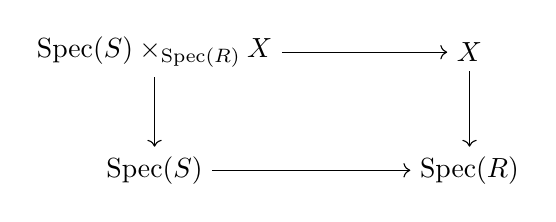
\begin{tikzpicture}
            \node (SX) at (0, 0) {$\Spec(S) \times_{\Spec(R)} X$};
            \node (S) at (0, -1.5) {$\Spec(S)$};
            \node (X) at (4, 0) {$X$};
            \node (R) at (4, -1.5) {$\Spec(R)$};

            \draw [->] (SX) -- (S);
            \draw [->] (SX) -- (X);
            \draw [->] (S) -- (R);
            \draw [->] (X) -- (R);
        \end{tikzpicture}
    \end{center}
    commute, is closed.
\end{corollary}
\begin{proof}
    Consider any scheme $Y$ over $\Spec(R)$.
    We have to show that the map $\pi: Y \times_{\Spec(R)} X \to Y$ that makes the diagram
    \begin{center}
        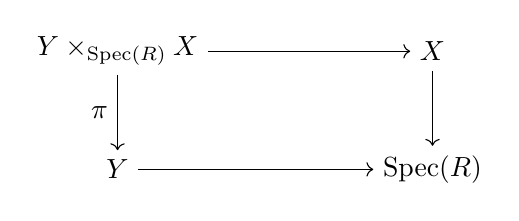
\begin{tikzpicture}
            \node (YX) at (0, 0) {$Y \times_{\Spec(R)} X$};
            \node (Y) at (0, -1.5) {$Y$};
            \node (X) at (4, 0) {$X$};
            \node (R) at (4, -1.5) {$\Spec(R)$};

            \draw [->] (YX) -- (Y) node [midway, left] {$\pi$};
            \draw [->] (YX) -- (X);
            \draw [->] (Y) -- (R);
            \draw [->] (X) -- (R);
        \end{tikzpicture}
    \end{center}
    commute, is closed.

    Let $Y = \bigcup_i V_i$ be a cover by affine opens.
    For each $i$, note that the diagram
    \begin{center}
        \begin{tikzpicture}
            \node (YX) at (0, 0) {$\pi^{-1}(V_i)$};
            \node (Y) at (0, -2) {$V_i$};
            \node (X) at (4, 0) {$X$};
            \node (R) at (4, -2) {$\Spec(R)$};

            \draw [->] (YX) -- (Y) node [midway, left] {$\pi_i := \restr{\pi}{\pi^{-1}(V_i)}$};
            \draw [->] (YX) -- (X);
            \draw [->] (Y) -- (R);
            \draw [->] (X) -- (R);
        \end{tikzpicture}
    \end{center}
    commutes.
    By the universal property of $V_i \times_{\Spec(R)} X$ we now find a morphism
    \begin{equation*}
        \psi: \pi^{-1}(V_i) \to V_i \times_{\Spec(R)} X
    \end{equation*}
    of schemes over $Y \times X$, i.e. the inclusion $\pi^{-1}(V_i)$ factors as
    \begin{equation*}
        \pi^{-1}(V_i) \ \overset{\psi}{\to} \ V_i \times_{\Spec(R)} X \ \to \ Y \times_{\Spec(R)} X
    \end{equation*}
    Considering $V_i \times_{\Spec(R)} X$ as an open subscheme of $Y \times_{\Spec(R)} X$, we thus see that $\psi$ must already be the identity and so $\pi^{-1}(V_i) \subseteq V_i \times_{\Spec(R)} X$.
    It follows that $\pi^{-1}(V_i) = V_i \times_{\Spec(R)} X$.

    By assumption we know that each $\pi_i$ is closed, as $V_i \cong \Spec(\O_Y(V_i))$ is affine.
    Now the previous lemma yields that also $\pi$ is closed.
\end{proof}
\begin{remark}
    \label{prop:functoriality_proj}
    Note that $\Proj$ is not functorial, in the sense that a homomorphism of graded rings $S \to T$ does not induce a natural morphism $\Proj(T) \to \Proj(S)$ (like $\Spec$ does).
    Namely, given $\alpha: S \to T$, we might want to consider
    \begin{equation*}
        \Proj(T) \to \Proj(S), \quad \p \mapsto \alpha^{-1}(\p)
    \end{equation*}
    However, in general this is not well-defined, as $\alpha^{-1}(\p)$ might contain $S_+$.

    If we further require the map $\alpha: S \to T$ to fulfill $T_+ \subseteq \alpha(S_+)T$, then this works out and we get a morphism
    \begin{align*}
        \Proj(\alpha): \Proj(T) &\to \Proj(S), \quad \p \mapsto \alpha^{-1}(\p), \\
        \Proj(\alpha)^\#_{D_f}: \O_{\Proj(S)}(D_f) &\to \O_{\Proj(T)}(D_{\alpha(f)}), \quad \frac x y \mapsto \frac {\alpha(x)} {\alpha(y)}
    \end{align*}
    Note that this is indeed a well-defined morphism, as for $\p \in \Proj(T)$ there is some $f \in T_+ \setminus \p$ and by assumption, have $g \in S_+, t \in T$ with $\alpha(g)t = f$.
    Now $g \notin \alpha^{-1}(\p)$, as $g \in \alpha^{-1}(\p)$ would imply $\alpha(g) \in \p$, thus $f = t\alpha(g) \in \p$.

    In particular, any ring homomorphism $R \to S$ induces a canonical morphism $\P_S^n \to \P_R^n$ of schemes, since the induced ring homomorphism $R[x_0, ..., x_n] \to S[x_0, ..., x_n]$ satisfies the above additional condition.
\end{remark}
\begin{lemma}
    \label{prop:projective_space_base_change}
    Let $R \to S$ be a ring homomorphism.
    Then the base change of $\P_R^n$ is
    \begin{equation*}
        \P_R^n \times_{\Spec(R)} \Spec(S) \cong \P_S^n
    \end{equation*}
    as schemes over $\Spec(S)$.
\end{lemma}
\begin{proof}
    Consider the canonical map $\alpha: R[x_0, ..., x_n] \to S[x_0, ..., x_n]$ induced by $R \to S$.
    Note that
    \begin{equation*}
        S \otimes_R (R[x_0, ..., x_n]_f)_0 \cong (S[x_0, ..., x_n]_{\alpha(f)})_0 \quad \text{via} \quad \iota_f: s \otimes \frac r {f^n} \mapsto \frac {s\alpha(r)} {\alpha(f)^n}
    \end{equation*}
    for all homogeneous $f \in R[x_0, ..., x_n]$.
    By Lemma~\ref{prop:Df_affine}, we see that $D_f$ for $f \in S[x_0, ..., x_n]$ homogeneous form an affine open cover of $\P_S^n$.
    Furthermore, we have a cover by affine opens $D_f \times_{\Spec(R)} \Spec(S)$ of $\P_R^n \times_{\Spec(R)} \Spec(S)$ for $f \in R[x_0, ..., x_n]$ homogeneous.
    Together, we see that it suffices to show that the isomorphisms (induced by $\iota_f$)
    \begin{equation*}
        \phi_f: D_{\alpha(f)} = \Spec((S[x_0, ..., x_n]_{\alpha(f)})_0) \to D_f \times_{\Spec(R)} \Spec(S)
    \end{equation*}
    glue to an isomorphism $\Proj(S[x_0, ..., x_n]) \to \P_R^n \times_{\Spec(R)} \Spec(S)$.
    By the gluing lemma, it suffices that the compatibility conditions are satisfied, i.e. that for all $f, g \in R[x_0, ..., x_n]$ homogeneous the diagram
    \begin{center}
        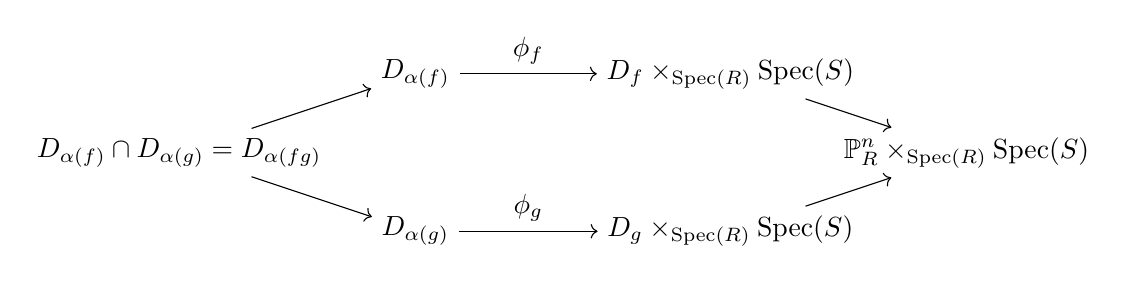
\begin{tikzpicture}
            \node (Sfg) at (0, 0) {$D_{\alpha(f)} \cap D_{\alpha(g)} = D_{\alpha(fg)}$};
            \node (Sf) at (3, 1) {$D_{\alpha(f)}$};
            \node (Sg) at (3, -1) {$D_{\alpha(g)}$};
            \node (f) at (7, 1) {$D_f \times_{\Spec(R)} \Spec(S)$};
            \node (g) at (7, -1) {$D_g \times_{\Spec(R)} \Spec(S)$};
            \node (all) at (10, 0) {$\P_R^n \times_{\Spec(R)} \Spec(S)$};

            \draw [->] (Sfg) -- (Sf);
            \draw [->] (Sfg) -- (Sg);
            \draw [->] (Sf) -- (f) node [midway, above] {$\phi_f$};
            \draw [->] (Sg) -- (g) node [midway, above] {$\phi_g$};
            \draw [->] (f) -- (all);
            \draw [->] (g) -- (all);
        \end{tikzpicture}
    \end{center}
    commutes.

    For a prime ideal $\p \in D_{\alpha(fg)}$ have that
    \begin{equation*}
        \phi_f(\p) = \iota_f^{-1}(\p \cap (S[x_0, ..., x_n]_f)_0) \in D_f \times_{\Spec(R)} \Spec(S)
    \end{equation*}
    and so $g \notin \phi_f(\p)$, i.e. $\phi_f(\p) \in D_{fg} \times_{\Spec(R)} \Spec(S)$.
    Hence, we have that both restrictions
    \begin{equation*}
        \restr{\phi_f}{D_{\alpha(fg)}}, \ \restr{\phi_g}{D_{\alpha(fg)}}: D_{\alpha(fg)} \to D_{fg} \times_{\Spec(R)} \Spec(S)
    \end{equation*}
    map into $D_{fg} \times_{\Spec(R)} \Spec(S)$.
    Now note that the diagram
    \begin{center}
        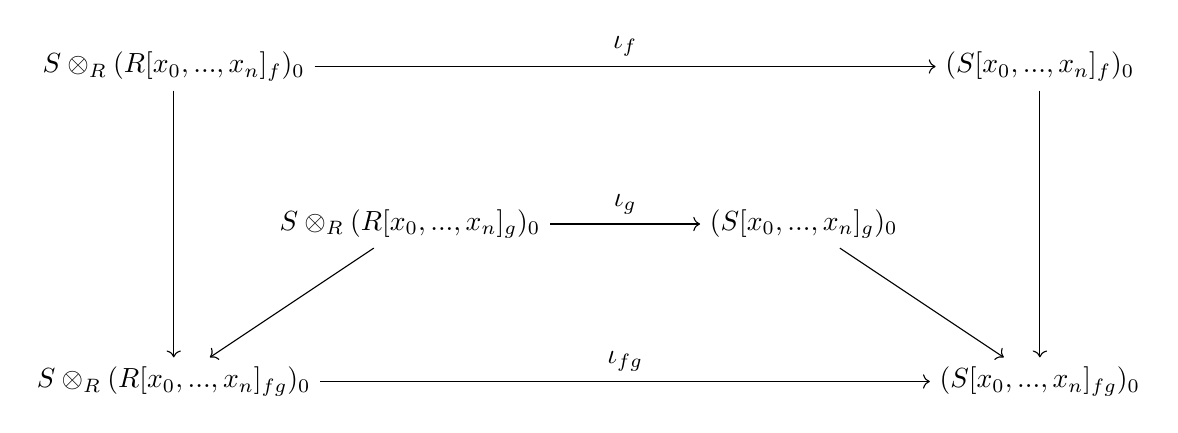
\begin{tikzpicture}
            \node (Rf) at (-3, 0) {$S \otimes_R (R[x_0, ..., x_n]_f)_0$};
            \node (Rg) at (0, -2) {$S \otimes_R (R[x_0, ..., x_n]_g)_0$};
            \node (Rfg) at (-3, -4) {$S \otimes_R (R[x_0, ..., x_n]_{fg})_0$};

            \node (Sf) at (8, 0) {$(S[x_0, ..., x_n]_f)_0$};
            \node (Sg) at (5, -2) {$(S[x_0, ..., x_n]_g)_0$};
            \node (Sfg) at (8, -4) {$(S[x_0, ..., x_n]_{fg})_0$};

            \draw [->] (Rf) -- (Sf) node [midway, above] {$\iota_f$};
            \draw [->] (Rg) -- (Sg) node [midway, above] {$\iota_g$};
            \draw [->] (Rfg) -- (Sfg) node [midway, above] {$\iota_{fg}$};

            \draw [->] (Rf) -- (Rfg);
            \draw [->] (Rg) -- (Rfg);
            \draw [->] (Sf) -- (Sfg);
            \draw [->] (Sg) -- (Sfg);
        \end{tikzpicture}
    \end{center}
    commutes, and so the restrictions of $\phi_f$ resp. $\phi_g$ to $D_{\alpha(fg)}$ are both induced by the homomorphism $\iota_{fg}$, hence they are equal.
    The claim follows.
\end{proof}
The next lemma is directly from \cite[II.4.5]{hartshorne}.
\begin{lemma}
    \label{prop:im_closed_iff_stable_specialization}
    Let $f: X \to Y$ be a quasi-compact morphism.
    Then $f(|X|)$ is closed if and only if it is stable under specialization.
\end{lemma}
\begin{lemma}
    \label{prop:adding_coeff_ideal_does_not_introduce_irrelevant_ideal}
    Let $\p \leq R[x_0, ..., x_n]$ be a homogeneous prime ideal with $R[x_0, ..., x_n]_+ \not\subseteq \p$.
    Further let $\q \leq R$ be a prime ideal such that $\p \cap R \subseteq \q$.
    Then there some $i$ such that no $\alpha x_i^m$ is in $\b := \p + \q R[x_0, ..., x_n]$, for any $\alpha \in R \setminus \b$ and any $m \in \N$.
\end{lemma}
\begin{proof}
    Assume there is $m \in \N$ such that $\alpha_i x_i^m \in \b$ for all $i$ and some $\alpha_i \in \b \setminus R$.
    Since $\b \cap R = \q$ is prime, have that $\alpha := \prod_i \alpha_i \notin \b$.
    Further we have that $\alpha x_i^m \in \b$ for all $i$.

    Consider now the vector $(w_i)_{i < N}$ containing all monomials of degree $(n + 1)m$.
    By assumption, all $\alpha w_i \in \b$.
    Since $\p$ is homogeneous, observe that now there are $r_{ij} \in \q$ such that
    \begin{equation*}
        \alpha w_i - \sum_{j < N} r_{ij} w_j \in \p
    \end{equation*}
    Working modulo $\p$, we see that $A w = \alpha w$ where $A \in (\b/\p)^{N \times N}$.

    Now observe that $\alpha \notin \b/\p$ since $\alpha \notin \b$.
    Hence there exists a prime ideal in $R/\p$ containing $\b/\p$ and not containing $\alpha$.
    Localizing at that prime ideal gives a local ring $S$ with maximal ideal $\mathfrak{l}$.
    Now assume that $w \in S^n$ and $A/\alpha \in \mathfrak{l}^{n \times n}$.
    Note that we still have $(A/\alpha) w = w$.

    wlog $S$ is noetherian, otherwise continue with the ring
    \begin{equation*}
        \tilde{S} := \begin{cases}
            \Z[A/\alpha, x] & \text{if $\mathrm{char}(S) = 0$} \\
            (\Z/\mathrm{char}(R)\Z)[A/\alpha, x] & \text{if $\mathrm{char}(S) \neq 0$}
        \end{cases}
    \end{equation*}
    generated by the coefficients of $A/\alpha$ and $w$ (this is noetherian, as it is a quotient of a polynomial ring in finitely many variables).
    
    Now equip $S_{\mathfrak{l}}$ with the $\mathfrak{l}$-adic topology.
    Note that $S$ is noetherian and local, thus the Krull intersection theorem shows that the $\mathfrak{l}$-adic topology is Hausdorff and we find
    \begin{equation*}
        w = \lim_{i \to \infty} w = \lim_{i \to \infty} \frac {A^i} {\alpha^i} w = \Bigl( \lim_{i \to \infty} \frac {A^i} {\alpha^i} \Bigr) w = 0 w = 0
    \end{equation*}
    since $(A/\alpha)^i$ has coefficients in $\mathfrak{l}^i$, thus converges to $0$ as $i \to \infty$.

    Thus $w \equiv 0 \mod \p$ and so $x_i^N \equiv 0 \mod \p$, i.e. $x_i^N \in \p$ for all $i$.
    However, since $\p$ is prime, this implies $R[x_0, ..., x_n]_+ = \langle x_0, ..., x_n \rangle \subseteq \p$, contradicting the assumption. 
\end{proof}
\begin{prop}
    \label{prop:projective_structure_morphism_closed}
    The morphism $\P_R^n \to \Spec(R)$ is closed.
\end{prop}
\begin{proof}
    Denote $\P_R^n \to \Spec(R)$ by $\phi$.
    Consider a closed set $\V(\a) = \P_R^n \setminus D_\a$ given by a homogeneous ideal $\a \leq R[x_0, ..., x_n]$.
    By Lemma~\ref{prop:im_closed_iff_stable_specialization}, it suffices to show that $\phi(\V(\a))$ is closed under specialization (note that $\P_R^n \to \Spec(R)$ is quasi-compact, e.g. by Proposition~\ref{prop:p_quasi_compact}).

    Consider $\q \in \phi(\V(\a)) \subseteq \Spec(R)$ and a prime ideal $\q'$ that specializes $\q$, i.e. $\q' \supseteq \q$.
    Then there is a $\p \in \V(\a)$ with $\p \cap R = \q$, in particular $\a \subseteq \p$.
    We want to show that $\q' \in \phi(\V(\a))$.

    Note that by Lemma~\ref{prop:adding_coeff_ideal_does_not_introduce_irrelevant_ideal}, there is $i$ such that the multiplicative set
    \begin{equation*}
        T := \{ \alpha x_i^m \ | \ \alpha \in R \setminus \q', \ m \in \N \}
    \end{equation*}
    has empty intersection with the ideal $\b := \p + \q' R[x_0, ..., x_n]$.
    
    Hence, the ring $T^{-1}(R[x_0, ..., x_n]/\b)$ is nonzero, thus has a prime.
    Taking its preimage under
    \begin{equation*}
        R[x_0, ..., x_n] \to R[x_0, ..., x_n]/\b \to T^{-1}(R[x_0, ..., x_n]/\b)
    \end{equation*}
    yields a prime ideal $\p'$ such that $x_i \notin \p'$ and $\b \subseteq \p'$.
    Clearly have that $\q' \subseteq \p'$ and since $\p' \cap T = \emptyset$, find that $\p' \cap R = \q'$.
    By Lemma~\ref{prop:homogeneous_part_prime}, assume wlog that $\p'$ is homogeneous.
    Now have a homogeneous prime ideal $\p'$ with $\a \subseteq \p \subseteq \p'$, i.e. $\p' \in \V(\a)$ and $\phi(\p') = \p' \cap R = \q'$.
    Thus $\q \in \phi(\V(\a))$ and the claim follows.
\end{proof}
\begin{corollary}
    The morphism $\P_R^n \to \Spec(R)$ is universally closed.
\end{corollary}
\begin{proof}
    Use Lemma~\ref{prop:universally_closed_affines}, so consider an affine base change $f_{\Spec(S)}: \P_R^n \times_{\Spec(R)} \Spec(S) \to \Spec(S)$.
    By Lemma~\ref{prop:projective_space_base_change}, have that $\P_R^n \times_{\Spec(R)} \Spec(S) \cong \P_S^n$ as schemes over $S$, hence $f_{\Spec(S)}$ is isomorphic to $\P_S^n \to \Spec(S)$.
    This morphism is closed by Proposition~\ref{prop:projective_structure_morphism_closed} and the claim follows.
\end{proof}
\begin{corollary}
    Projective space $\P_R^n$ over $\Spec(R)$ is proper.
\end{corollary}
\begin{corollary}
    Let $k$ be an algebraically closed field.
    Then projective space $\P_k^n$ over $\Spec(k)$ is a complete variety.
\end{corollary}

\section{Valuative criterion of properness}
\begin{prop}
    Let $X$ be noetherian and $f: X \to Y$ a morphism of finite type.
    The following are equivalent
    \begin{itemize}
        \item $f$ is proper
        \item For every valuation ring $R$ with field of fractions $K = \Frac(R)$ and all morphisms $\Spec(R) \to Y$, $\Spec(K) \to X$ that make the diagram
        \begin{center}
            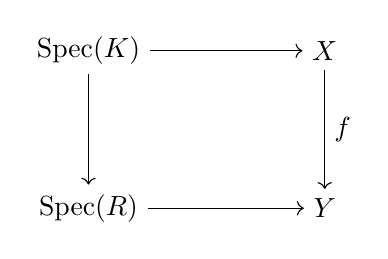
\begin{tikzpicture}
                \node (K) at (0, 0) {$\Spec(K)$};
                \node (R) at (0, -2) {$\Spec(R)$};
                \node (X) at (3, 0) {$X$};
                \node (Y) at (3, -2) {$Y$};
    
                \draw [->] (K) -- (R);
                \draw [->] (K) -- (X);
                \draw [->] (R) -- (Y);
                \draw [->] (X) -- (Y) node [midway, right] {$f$};
            \end{tikzpicture}
        \end{center}
        commute, there exists a unique compatible morphism $\Spec(R) \to X$.
    \end{itemize}
\end{prop}
\printbibliography
\end{document}